\chapter{Method}
\label{sec:method}
As explained in \Cref{sec:introduction} the aim of this work is to find a drone
design that is the result of an optimization problem, which tends to maximize the
MAV's omni-directionality, flight efficiency and controllability. To do so it is
important to first state what are the parameters that define the design of an MAV.
These parameters are defined as:

\begin{itemize}
\item $\beta$  (angles formed by the arms with the horizontal plane see \Cref{fig:drone_design})
\item $\theta$ (angles formed by the arms in the horizontal plane see \Cref{fig:drone_design})
\item L (arm length)
\item n (number of propeller)
\end{itemize}

\begin{figure}[h]
\centering
\begin{minipage}[t]{0.3\textwidth}
  \centering
  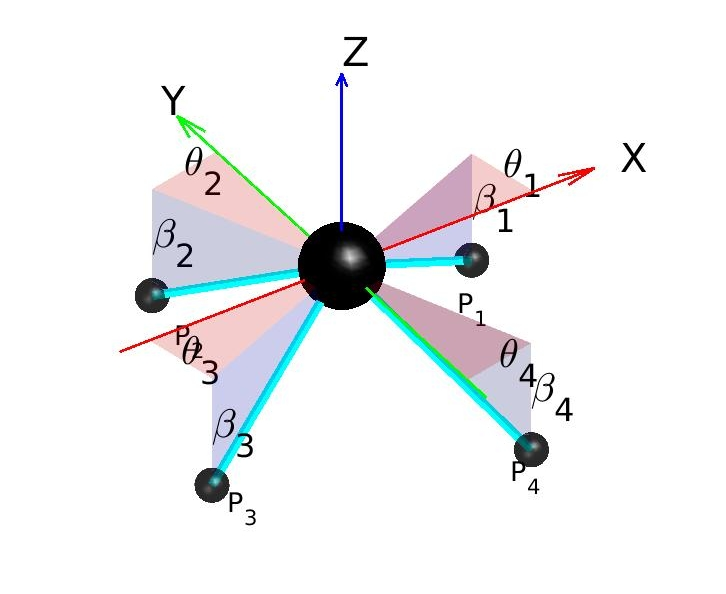
\includegraphics[width=\textwidth]{images/drone_design.jpg}
\end{minipage}
\hfill
\begin{minipage}[t]{0.3\textwidth}
  \centering
  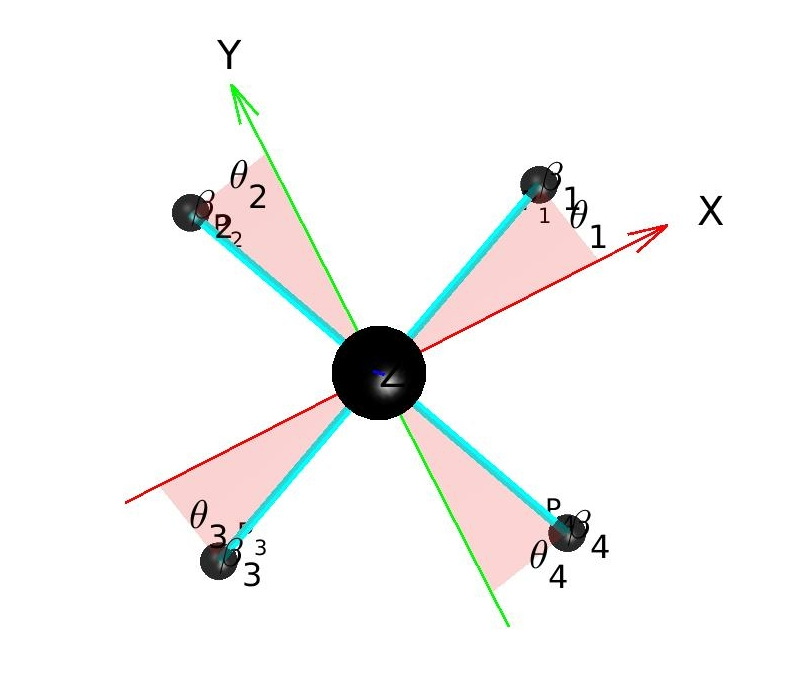
\includegraphics[width=\textwidth]{images/drone_design1.jpg}
\end{minipage}
\hfill
\begin{minipage}[t]{0.3\textwidth}
  \centering
  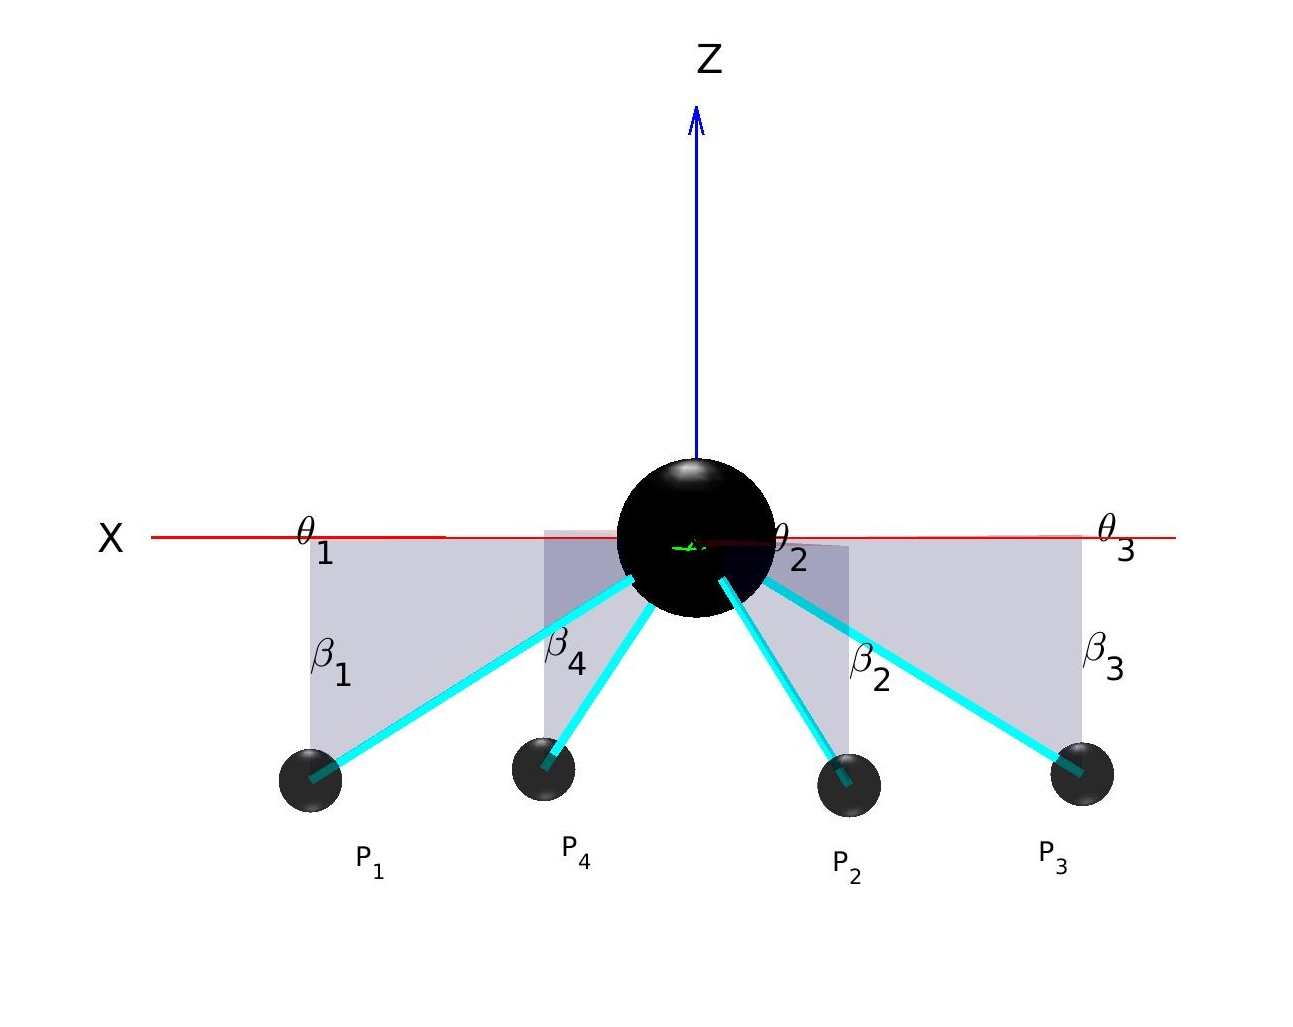
\includegraphics[width=\textwidth]{images/drone_design2.jpg}
\end{minipage}
\caption{Quadcopter to illustrate the parameters that define the morphology of an
MAV ($n = 4$, $\beta = [30, 30, 30, 30] [^{\circ}]$, $\theta = [22, 22, 22, 22]
[^{\circ}]$, and $L = 0.4 [m]$).}
\label{fig:drone_design}
\end{figure}

To solve the problem an optimization engine is developed with
Matlab$^\textrm{\textregistered}$. This tool returns the aforementioned
parameters along with other information on the corresponding MAV design.
The interesting drone designs outputted by the tool are then simulated on
Gazebo\footnote{An open source robot simulator \citep{noauthor_gazebo_nodate}.}
and the control of the different models is achieved using a Robotic Operating
System\footnote{An open source collection of software that help developers to
create robot applications \citep{rostutorials}.} (ROS) node.\\
This chapter first covers the theory needed to obtain a generalize mathematical
model for a n-rotor MAV with an arbitrary morphology. Then, the optimization
problem is defined. Afterwards, the optimization tool is described. In the end,
the theoretical background needed to perform the simulations is covered.

\section{Modelisation of MAVs}
\label{sec:modeling_mav}
In the following part, a dynamical model for a general design of MAV is presented.
This model is inspired from the models presented in \citep{kamel_voliro:_2018} and
\citep{ryll_modeling_2012}.

\subsubsection{Initial Definitions}
\label{sec:definitions}
In order to understand correctly the dynamical model, a few definitions are much
needed. First, let us define $\mathcal{F}_{W} : \{O_{W}; X_{W},  Y_{W},  Z_{W}\}$
as the world fixed inertial frame and $\mathcal{F}_{B}: \{O_{B}, X_{B},  Y_{B},
Z_{B}\}$
as a moving frame attached to the MAV. Also, $\mathcal{F}_{P_{i}} : \{O_{P_{i}};
X_{P_{i}}, Y_{P_{i}},  Z_{P_{i}}\}, i = 1...n$ is the frame of the i-th propeller.
The propeller rotate around the axis $Z_{P_{i}}$, and thus the thrust $T_{i}$ is
produced along this axis. The tilt movement of the rotors is a simple rotation
around $X_{P_{i}}$. Now let $^{W}R_{B}$ be the orientation of the body frame
with respect to the world frame and $^{B}R_{P_{i}}$ be the orientation of the
i-th propeller with respect to the body frame. From there, it
straightforward with the help of \Cref{fig:tilt_model} that

\begin{equation}
  \label{rot_b_pi}
  ^{B}R_{P_{i}} \ = \ R_{Z}\bigg((i-1)\frac{2\pi}{n}\bigg) R_Z(\theta_i)
  R_Y(\beta_i) R_{X}(\alpha_{i}),\  i = 1...n\, .
\end{equation}

Equivalently, let

\begin{equation}
  \label{O_pi}
  ^{B}O_{P_{i}} \ = \ R_{Z}\bigg((i-1)\frac{2\pi}{n}\bigg) R_Z(\theta_i) R_Y(\beta_i)
  \begin{bmatrix}
    L \\
    0 \\
    0
  \end{bmatrix}
  ,\   i = 1...n \,
\end{equation}

be the origin of the i-th propeller frame  $\mathcal{F}_{P_{i}}$.
In \Cref{rot_b_pi} and (\ref{O_pi}), $(i-1)\frac{2\pi}{n}$ is the angle that
the i-th arm would form with axis $X_B$ if the arms of the drone are evenly
distributed in the horizontal plane, $\theta_i$ is the angle that i-th arm forms
in the horizontal plane with respect to its evenly distributed position
(see \Cref{fig:drone_design}), $\beta_i$ is the angle that the i-th arm forms with
the horizontal plane (see \Cref{fig:drone_design}), $\alpha_{i}$ is the tilting
angles of the i-th propeller about the $X_{P_{i}}$ axis, L is the arm length and
n is the number of propellers.

\begin{figure}[h]
  \centering
  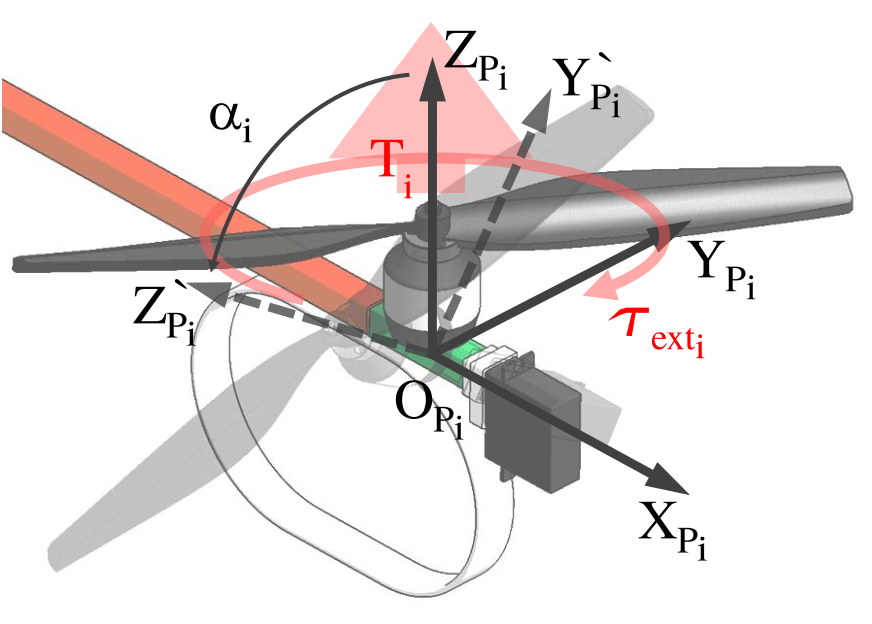
\includegraphics[width=0.5\textwidth]{images/tilt_model.png}
  \caption{Representation of the i-th tilting arm \citep{ryll_modeling_2012}.}
  \label{fig:tilt_model}
\end{figure}

\subsubsection{Assumptions}
\label{sec:assumptions}
In this model the first assumption is that the MAV is composed of n+1 rigid bodies:
one for each propeller $P_i$ and one for the body B. Then, it is considered that
the motors that actuate the propellers can only rotate in one direction. Finally,
the airflow interactions between the different rotors are neglected.

\subsubsection{Equations of motion}
\label{sec:equations}
Using Newton-Euler formalism, it follows that
\begin{equation}
  \label{acc_eq}
  \begin{cases}
    \dot{\omega}_B  \ = \ I_B^{-1} \sum_{n=1}^{n}  \big(\ ^{B}O_{P_{i}} \tau_{ext,i} + \tau_{Bi} \ \big) \, ,\\
    \ddot{p}  \ = \
    \begin{bmatrix}
      0 \\
      0 \\
      g
    \end{bmatrix}
    \ ^{W}R_B \sum_{n=1}^{n} T_i \, .
  \end{cases}
\end{equation}

Where

\begin{equation}
  \label{tau_b_i}
  \tau_{Bi}  \ = \ ^{B}O_{P_{i}} \times\   ^{B}R_{P_{i}} T_{P,i}
\end{equation}

\begin{equation}
  \label{tau_ext_i}
  \tau_{ext,i}  \ = \  \big[0 \ \  0 \ \  - c_i \kappa_m w_i^2 \big]^T \
  \begin{cases}
    c_i = 1, & \mbox{if } i \mbox{ is odd } (cw\ rotation)\\
    c_i = -1 & \mbox{if } i\mbox{ is even } (ccw\ rotation)
  \end{cases}
\end{equation}

and

\begin{equation}
  \label{T_i}
  T_i  \ = \ ^{B}R_{P_{i}} T_{Pi} \, ,\ \ T_{Pi}  \ = \ \big[0 \ \ 0 \ \
  \kappa_f w_i^2 \big]^T\, .
\end{equation}




\section{Optimization problem}
\label{sec:optimization_problem}
Define morphology optimization problem

\section{Optimization tool}
\label{sec:optimization_tool}
Show resulting optimization tool.

\section{Simulation Approach}
\label{sec:control_approach}
